% Author - - Jon Arnt Kårstad, NTNU IMT
\documentclass{article}

% Importing document settings from our file "packages.sty"
\usepackage{packages}

% Beginning of document
\begin{document}

% Inserting title page
\import{./}{title}

% Defining front matter settings 
\frontmatter

% Inserting table of contents
\tableofcontents

% Inserting list of figures & list of tables
\listoffigures
\listoftables

% Defining main matter settings
\mainmatter

\section{Motivation}
    \import{./Sections/}{Motivation}

\section{Grundlagen}
    \import{./Sections/Introduction}{Introduction}

    \subsection{OOP Design Patterns}
        \import{./Sections/Introduction/OOPDesignPatterns}{OOPPatterns}

        \subsubsection{Observer}
            \import{./Sections/Introduction/OOPDesignPatterns/sub/}{Observer}

        \subsubsection{Proxy}
            \import{./Sections/Introduction/OOPDesignPatterns/sub/}{Proxy}

        \subsubsection{TemplateMethod}
            \import{./Sections/Introduction/OOPDesignPatterns/sub/}{TemplateMethod}

        \subsubsection{Builder}
            \import{./Sections/Introduction/OOPDesignPatterns/sub/}{Builder}

        \subsubsection{Facade}
            \import{./Sections/Introduction/OOPDesignPatterns/sub/}{Facade}

    \subsection{Architecturen}
        \subsubsection{Clean Architectur}
            \import{./Sections/Introduction/CleanArchitecture}{CleanArchitecture}
        \subsubsection{Model-View Architekturen}
            lol kek cheburek

    \subsection{Software Testing}
        \import{./Sections/Introduction/SoftwareTesting}{SoftwareTesting}

        \subsubsection{Testing Pyramide}
            \import{./Sections/Introduction/SoftwareTesting/sub/}{TestingPyramide}
        
        \subsubsection{Unit Tests}
            \import{./Sections/Introduction/SoftwareTesting/sub/}{UnitTests}
        
        \subsubsection{Integration Tests}
            \import{./Sections/Introduction/SoftwareTesting/sub/}{IntegrationTests}

        \subsubsection{SystemTests}
            \import{./Sections/Introduction/SoftwareTesting/sub/}{SystemTests}

        \subsubsection{UI Tests}
            \import{./Sections/Introduction/SoftwareTesting/sub/}{uitests}

        \subsubsection{Manual Tests}
            \import{./Sections/Introduction/SoftwareTesting/sub/}{ManualTests}

    \subsection{SOLID}
        \import{./Sections/Introduction/SOLID/}{SOLID}

        \subsubsection{single-responsibility principle}
            \import{./Sections/Introduction/SOLID/sub/}{SingleResponsibilityPrinciple}
        
        \subsubsection{open–closed principle}
            \import{./Sections/Introduction/SOLID/sub/}{OpenClosedPrinciple}
        
        \subsubsection{Liskov substitution principle}
            \import{./Sections/Introduction/SOLID/sub/}{LiskovSubstitutionPrinciple}
        
        \subsubsection{interface segregation principle}
            \import{./Sections/Introduction/SOLID/sub/}{InterfaceSegregationPrinciple}
        
        \subsubsection{dependency inversion principle}
            \import{./Sections/Introduction/SOLID/sub/}{DependencyInversionPrinciple}

    \subsection{GRASP}
        \import{./Sections/Introduction/GRASP/}{GRASP}

    \subsection{OOP Principles}
        \import{./Sections/Introduction/OOPPrinciples/}{OOPPrinciples}

        \subsubsection{Abstraction}
            \import{./Sections/Introduction/OOPPrinciples/sub}{Abstraction}

        \subsubsection{Encapsulation}
            \import{./Sections/Introduction/OOPPrinciples/sub}{Encapsulation}

        \subsubsection{Inheritance}
            \import{./Sections/Introduction/OOPPrinciples/sub}{Inheritance}

        \subsubsection{Polymorphism}
            \import{./Sections/Introduction/OOPPrinciples/sub}{Polymorphism}

\newpage

\section{Software Architektur}
    \subsection{Was ist eine Software Architektur}

    Bevor man anfängt über die Software Architektur zu reden, muss man sie erstmal definieren.
    Es gibt keine einheitliche Definition einer Software Architektur. Verschiedene Authoren definieren es auch unterschiedlich.

    Robert Martin definiert es als ein Gegenstand mit bestimmten Eigenschaften zu definieren.\\
    \textit{Softwarearchitektur ist die Gestalt des Systems erstellt von derjenigen, die das entwickeln. 
    Die Form dieser Gestalt ist das Aufteilen des Systems in Komponenten, die Anordnung (Arrangement) dieser Komponenten und die Wege, 
    wie diese Komponente miteinander kommunizieren} \cite[136]{cleanArchitecture}
    
    Ralph Jonson definiert Software Architektur aus Sicht eines Projektes.\\
    \textit{Architektur besteht aus den Entscheidungen, die man sich wünscht so früh wie möglich in einem Projekt zu treffen}
    \cite{MF_WhatIsSA}

    In dem ersten Teil des Kapitels wird die Softwarearchitektur aus Sicht eines Projektes betrachtet, 
    indem es kurz beschrieben wird, welche Auswirkungen eine gute und eine schlechte Architektur auf ein Projekt haben kann.

    In dem 2. Teil des Kapitels, wird die Architektur des OCPP Backend Servers beschrieben
    \begin{itemize}
        \item Aufteilung des Programms in einzelne Teile
        \item Testbarkeit und Erweitbarkeit einzelner Teile des Programms
        \item Kommunikation zwischen den einzelnen Teilen
    \end{itemize}

    \subsection{Ziele der Software Architektur}

    \textit{Das Ziel der Software Architektur ist das Mininimieren der menschlichen Ressourcen, 
    die benötigt werden um ein System zu entwickeln und zu unterstützen.}\cite[5]{cleanArchitecture}

    Diese Aussage lässt sich sehr einfach überprüfen, indem man feststellt, 
    ob jede neue Anforderungen an der Software mehr Ressourcen verbraucht als die vorherigen.

    \textit{Das Ziel der Softwarearchitektur ist so viel Entscheidungen wie möglich so spät wie möglich zu treffen}
    \cite[136]{cleanArchitecture}

    Beispiele für solche Entscheidungen wären:
    \begin{itemize}
        \item Datenbanksystem
        \item Transferprotokoll zu der Benutzeroberfläche (z.B. HTTP oder WS) falls vorhanden
        \item Wie und wo die Loggingdaten gespeichert werden (in einer Datei, Datenbank oder externe Server)
    \end{itemize}

    Auch die Tätigkeiten, die nicht mit Programmieren direkt zu tun haben, werden von den Entscheidungen in der Softwarearchitektur betroffen
    \begin{itemize}
        \item Deployment (Aufsetzung) der Software.
        \item Maintenance (Unterstützung) der Software.
    \end{itemize}

    Deployment der Software beinhaltet die Kosten die durch das Aufsetzen der neuen Version der Software entstehen.\\
    Maintenance der Software beinhaltet die Kosten, die nach dem Beenden der Entwicklung bei kleineren Erweiterungen und Änderungen des Systems entstehen.


    \subsection{Technische Schulden}
    Bei den Änderungen oder Erweiterungen eines Systems oft entsteht ein Overhead, das durch die ``Unsaubarkeit'' des bestehenden Programms verusacht wird.

    Dieses Overhead wird als technische Schulden (en. : Technical Debts) bezeichnet.

    Die technischen Schulden entstehen dadurch, dass bei der Entwicklung eines Teiles des Systems wurde 
    von den Entwicklungsteam weniger Zeit investiert um die nicht gewinnbringende Aufgaben zu erledigen.
    Beispiele für solche Tätigkeiten wären:
    \begin{itemize}
        \item Unittests
        \item Dokumentieren 
        \item Code Review
    \end{itemize}

    Beispiele für Technische Schulden wären:
    \begin{itemize}
        \item Alte Funktionalitäten funktionieren nach der Änderung nicht mehr
        \item Aufdeckung eines Bugs erst nach einer gewissen Zeit in Produktionsversion der Software
        \item Implementieren der neuen Funktionalitäten verbraucht deutlich mehr Zeit
    \end{itemize}

    Eine klare Struktur der Software reduziert die Menge an technischen Schulden, 
    die die Weiterentwicklung in der Zukunft verlangsamen. 

    Die Softwareentwickler können die ankommenden Aufgaben erledigen
    \begin{itemize}
        \item man hat bereits Vorgaben wie die Kommunikationswege zwischen den Modulen ist
        \item wie die Module benannt werden sollen
        \item an welchen Stellen das Modul in das System hinzugefügt werden soll
        \item die Menge an durch den "Zufall" entstehenden Bugs in anderen Teilen des Programms ist minimal
    \end{itemize}

    Durch die bereits definierten Kommunikationswege zwischen den Modulen, muss weniger Dokumentation geschrieben werden.
    Mit weniger Dokumentation findet man schneller die gesuchten Informationen.

    Durch die einheitliche Bezeichnung der Teile des Modules kann man allein aus dem Namen des Modules seine Aufgaben ableiten.

    Daher ist es vom Vorteil bevor man mit der Umsetzung des Softwaresystems anfängt, die oben gennanten Aufgaben zu lösen,
    denn mit zunehmender Lebenszeit der Software nimmt die Änderungszeit zu.

    Somit lassen sich die vorhandenen Ressourcen effizienter eingesetzen.

    \newpage
    \subsection{Qualität und Kosten der Software}
    \nocite{MF_isHighQuilatySoftwareWorthTheCost}

    Am Anfang jedes neuen Projektes in der Softwareentwicklung muss die Entscheidung getroffen werden, wie qualitativ gut die Software am Ende sein soll.
    Damit sind die Eigenschaften/Funktionalitäten der Software gemeint, die für die Benutzer irrelevant sind, jedoch eine sehr große Bedeutung 
    für das Entwicklungsteam haben.
    
    Wenn man eine qualitativ gute Software hat, ergeben sich unteranderem folgende Vorteile:
    \begin{itemize}
        \item Bugs können schneller lokalisiert und beseitigt werden
        \item Neue Funktionalitäten können mit weniger Aufwand umgesetzt werden
        \item Die Änderungen der Funktionalitäten können schneller umgesetzt werden
        \item Die Wahrscheinlichkeit bestehende Funktionalitäten ungewollt zu ändern veringert sich
        \item Die Einarbeitungszeit von neuen Teammitgliedern verkürzt sich 
    \end{itemize}

    Alle diese Vorteile hat man nicht kostenlos, denn dafür muss man auch Zeit investieren indem man:
    \begin{itemize}
        \item Regelmäßig die Software refactored
        \item Code Qualität überprüft
        \item Code Reviews durchführt
        \item Automatisierte Tests schreibt (Unit-, Integration- und Systemtests)
        \item Dokumentation aktuell hält
        \item Die technischen Schulden gering hält
    \end{itemize}

    Nicht in jedem Projekt ist das Umsetzen von oben genannten Eigenschaften möglich, 
    denn man hat nicht genug Zeit oder das Budget ist zu klein dafür.
    Man kann aber gewisse Kriterien setzen um mit deren Hilfe bessere Entscheidung zu treffen:
    \begin{itemize}
        \item Wann soll die MVP\footnote[1]{Minimum viable product} vorhanden sein.
        \item Wie viele Ressourcen man zur Verfügung hat
        \item Wie wahrescheinlich sind die Änderungen und Erweiterungen der Software
        \item Wie kritisch verschiede Probleme und Ausfälle der Software sind 
    \end{itemize}

    Auf dem unterer Darstellung sieht man, dass auf langere Distanz eine gute Softwarearchitektur deutlich
    mehr Funktionalitäten besitzt als eine Software mit schlechter Architektur. 
    Jedoch es gibt einen Zeitinterval, in dem die schlectere Software besser da steht.
    \begin{figure}[H]
        \centering
        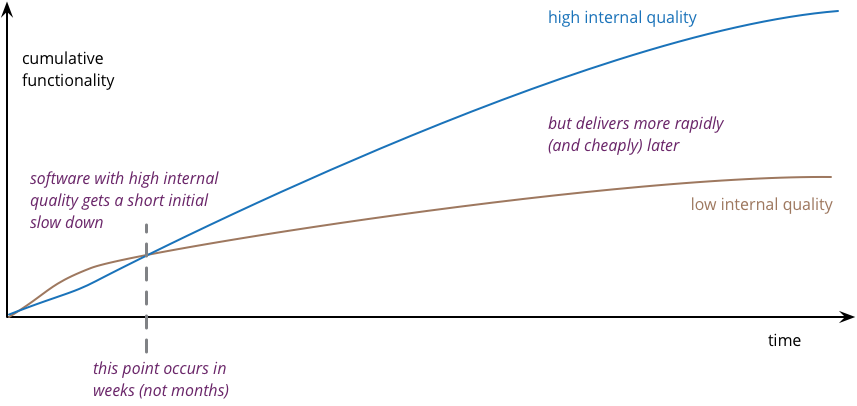
\includegraphics[width=1\textwidth]{./images/QASoftwareCompare.png}
        \caption[Vergleich einer guten und einer schlechten Softwarearchitektur]{Vergleich einer guten und einer schlechten Softwarearchitektur \footnotemark}
        \label{fig:softQuality}
    \end{figure}
    \footnotetext{https://martinfowler.com/articles/is-quality-worth-cost.html}
    Diese Eigenschaft muss man immer beim Projektbegin beachten, denn es wäre Zeitaufwändig für ein Studiumprojekt, 
    für das man evtl. nur eine Woche Zeit hat, um eine komplexe Architektur zu implementieren, die ohne jeglichen Funktionalitäten mehrere Wochen gebrauchen wird.

    Wenn man aber ein Projekt hat, das regelmäßig weiterentwickeln wird, ist es vom Vorteil gleich eine gute Architektur umzusetzen.

    \subsection{Wichtigkeit der Testbarkeit der Software}
    Jedes Teil der Software wird in seinem Lebenszyklus mehrmals geändert. 
    Um die Funktionalität der neuen Version zu verifizieren, muss sie getestet werden.
    Es ist von Interesse diese Aufgabe zu automatisieren. 
    Wie in den früheren Kapitels bereits beschrieben wurde, am schnellsten findet man die Bugs, falls vorhanden, mit Unittests. 
    Bei den Unittests müssen die Module (z.B. einzelne Klassen in Falle von OOP Sprachen) in verschiedenen Umgebungen überprüft werden. 
    Das heißt, dass die Zustände von benutzten Modulen müssen einfach zu simulieren sein.
    Dies erfordert eine Planung der Softwarearchitektur im Voraus, 
    um diese Eigenschaft zu implementieren um im Laufe der Entwicklung, Zeit durch automatisierte Tests zu sparen.

    \newpage
    \subsection{Technische Umsetzung der Software Architektur}

    Der OCPP Backend Server wurde anhand ``Clean Architecture'' projektiert und entsprechend umgesetzt. 
    Im Kapitel werden die benutzten Schichten beschrieben, welche Eigenschaften sie besitzen und wie sie miteinander verbunden sind.
    Auch wird kurz gezeigt wie es mit der Testbarkeit auf allen Niveaus (Unit, Integration und Systemtests), 
    Änderbarkeit und Erweitbarkeit der Software ist.

    \import{./images/}{circle_1}
    \footnotetext{Eigene Quelle}

    Beschreibung der Darstellung:
    Jede Komponente bringt in das gesamt Programm folgende Teile:
    \begin{itemize}
        \item Port - z.B. WebSocket Server aufzubauen
        \item Adapter  - umwandeln der ankommenden Nachrichten bzw. Ereignisse in die Typen definierten im Domain
        \item Controller - definiert alle Tätigkeiten, die die Komponente machen könnte
        \item UseCase - definiert den Ablauf an Tätigkeiten (Interactoren) beim Geschehen eines Ereignisses
        \item Interactors - Hülle für alle definierten Tätigkeiten im Controller
        \item Domain - definiert Typen benutzten der Komponente und deren Basic Verhalten, auch die Ereignisse die vom Dispatcher verteilt werden
    \end{itemize}

    \newpage
    \subsection{Abhängigkeiten im Programm}

    Die Architektur lässt sich in zwei wesentlichen Teilen zerlegen
    \begin{itemize}
        \item Anbindung an Infrastruktur um das Programm (Port - Adapter - Controller)
        \item Innere Logik des Programms (Controller - Dispatcher - UseCase - Interactor)
    \end{itemize}

    Beispiele für die Infrastruktur sind: Datenbank, Persistenz, Schnittstellen (HTTP, USB usw)

    Bei solcher Aufteilung ergeben sich folgende Vorteile:
    \begin{itemize}
        \item Innere Logik des Programms lässt sich mittels Integrationstests unabhängig von Schnittstellen abdecken.
        Damit ist die Laufzeit von jedem einzelnen Test ohne reelen Schnittstellen ist schneller als mit reelen Schnittstellen und 
        man hat das gleiche Ergebnis bezüglich des Verhaltens des Programms.
        \item Die Innere Logik ist nicht an Schnittstellen gebunden, 
        somit können alle Schnittstellen mit wenig Aufwand getauscht werden.
    \end{itemize}

    \subsubsection{Port-Adapter-Controller}
    \label{Port-Adapter-Controller}
    Am nähesten zu der \textbf{PAC}\footnote{Port-Adapter-Controller} Struktrur 
    ist das Pattern \textbf{MVP}\footnote{Model-View-Presenter}.
    Dabei die Aufgaben von \textbf{View} entsprechen den Aufgaben von \textbf{Port}. 
    Die Aufgaben von \textbf{Presenter} entsprechen den Aufgaben \textbf{Adapter}.
    Und die Aufgaben von dem Rest des Programms inklusiv \textbf{Controller} entspechen den Aufgaben von \textbf{Model}.

    Der Unterschied zu \textbf{MVP} besteht darin, dass \textbf{MVP} im klassischen Sinne nur für die Benutzerobeflächen gedacht ist,
    während in der hier beschriebenen Umsetzung wird es für alle Schnittstellen benutzt.
    \textbf{MVP} Architektur übernimmt in der gesamten Application eine zentralle Stelle und ist nur einmal zu treffen.
    \textbf{PAC} ist nur ein Teil der gesamten Application, wird an mehreren Stellen unterschiedlich benutzt und beschreibt nicht 
    die Architektur der Application.


    \begin{figure}[H]
       \centering
       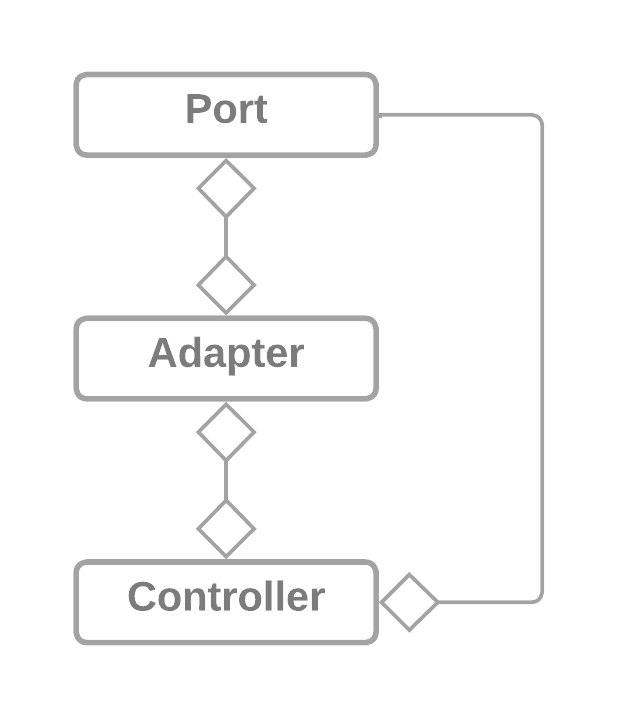
\includegraphics[width=6.5cm]{./images/Port-Adapter-Contoller.png}
        \caption[Klassendiagrammm PAC]{Klassendiagrammm PAC \footnotemark}
        \label{fig:CDPAC}
    \end{figure}
    \footnotetext{Eigene Quelle}

    \subsubsection{Controller-Dispatcher-UseCase-Interactor} 
    \label{Controller-Dispatcher-UseCase-Interactor}
    In dem Teil wird die komplete innere Logik der Application beschrieben. Dafür ist nur \textbf{Controller} notwendig. 
    D.h. beim Geschehen eines Ereignisses wird eine (oder mehrere) Method(en) in deb jeweiligen Controllern aufgerufen,
    die das Ereignis entsprechend abarbeiten.
    Dabei hat man folgendes Problem:
    jeder \textbf{Controller} übernimmt mehrere Aufgaben 
    (z.B. Kontrollieren von \textbf{Port} und \textbf{Adapter} und enthält Anwendungslogik)
    d.h. keine \textbf{SRP}

    Eine mögliche Lösung wäre das Separieren von Kontrollieren von \textbf{Port} und \textbf{Adapter} und Anwendungslogik
    in 2 verschiedenen Teile. Die Anwendungslogik heißt \textbf{UseCase}.

    Bei dieser Aufteilung besteht das Problem, dass beim Geschehen eines Ereignisses im \textbf{Controller} muss dieses Ereignis an das 
    richtige \textbf{UseCase} zugeordnet werden. D.h. \textbf{Contoller} besitzt eine weitere Verantwortlichkeit die sich in ein anderes Teil
    verschieben lässt. Dieses Teil heißt \textbf{Dispatcher}, dessen Aufgabe ist das Informieren alle daran Interessierten \textbf{UseCase}s
    beim Geschehen eines Ereignisses. 

    Jedes \textbf{UseCase} kann mehrere aufeinander folgende Aufgaben machen.
    Alle Aufgaben müssen gleiche Funktionalitäten besitzen, z.B:
    \begin{itemize}
        \item der Anfang und das Ende in Logs aufzeichnen.
        \item Nach einer bestimmten Zeit gestoppt werden.
    \end{itemize}
    D.h. man braucht eine ``Hülle'' um jeder Methode - \textbf{Interactor}

    Wenn man das alles zusammen entsteht folgendes Klassendiagrammm:

    \begin{figure}[H]
        \centering
        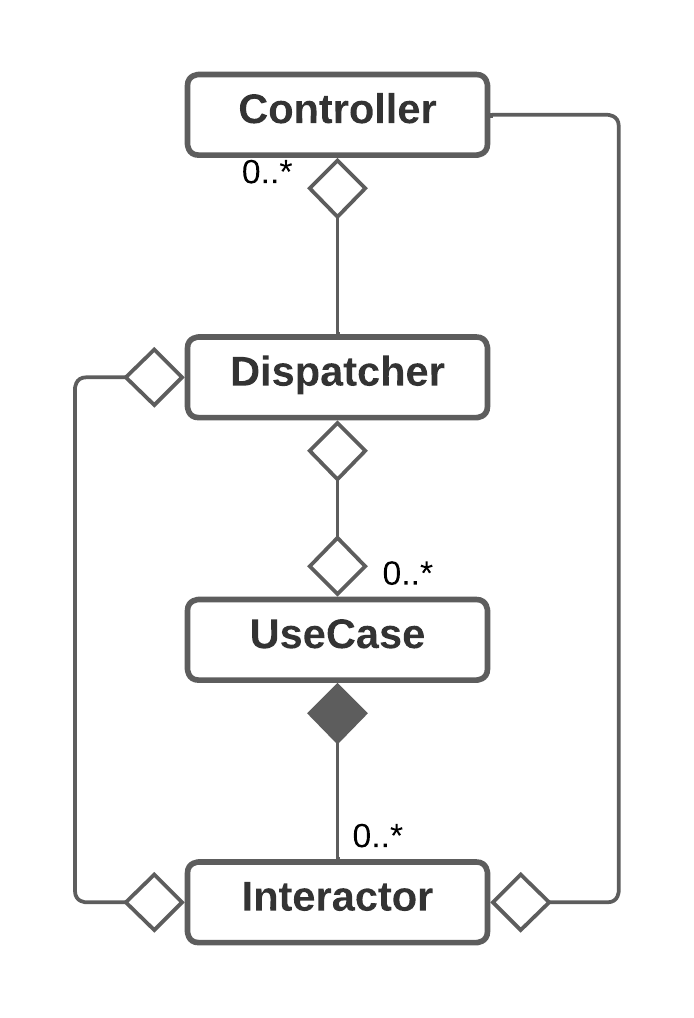
\includegraphics[width=6.5cm]{./images/Controller-Dispatcher-UseCase-Interactor.png}
         \caption[Klassendiagrammm Controller-Dispatcher-UseCase-Interactor]{Klassendiagrammm Controller-Dispatcher-UseCase-Interactor \footnotemark}
         \label{fig:CDCDUI}
    \end{figure}
    \footnotetext{Eigene Quelle}

    \newpage
    \subsubsection{Erstellen der Struktur}
    In den Kapiteln \ref{Controller-Dispatcher-UseCase-Interactor} und \ref{Port-Adapter-Controller} 
    werden die fertigen Strukturen beschrieben, diese Strukturen müssen am Anfang des Programms erstellt
    und miteinander verbunden werden.

    Das Erstellen von der Struktur findet im \textbf{Main} statt und lässt sich in drei Schritte aufteilen:
    \begin{itemize}
        \item Erstellen alle Instanzen
        \item Verknüpfen alle Instanzen miteinander
        \item Starten alle Instanzen
    \end{itemize}

    Das Erstellen aller Instanzen lässt sich in zwei weitere Schritte aufteilen, die bedingt voneinander abhängen.
    \begin{itemize}
        \item Core (Controllers + Dispatcher + UseCases + Interactors)
        \item Schnittstellen (Port + Adapter + Controller)
    \end{itemize}

    Damit auch Integrationstests für den kompleten Core und jede Schnittstellen möglich sind, wäre es sinnvol, dass beide Schritte
    explicit ausgeführt werden.

    Ein möglicher Ablauf wäre:
    \begin{figure}[H]
        \centering
        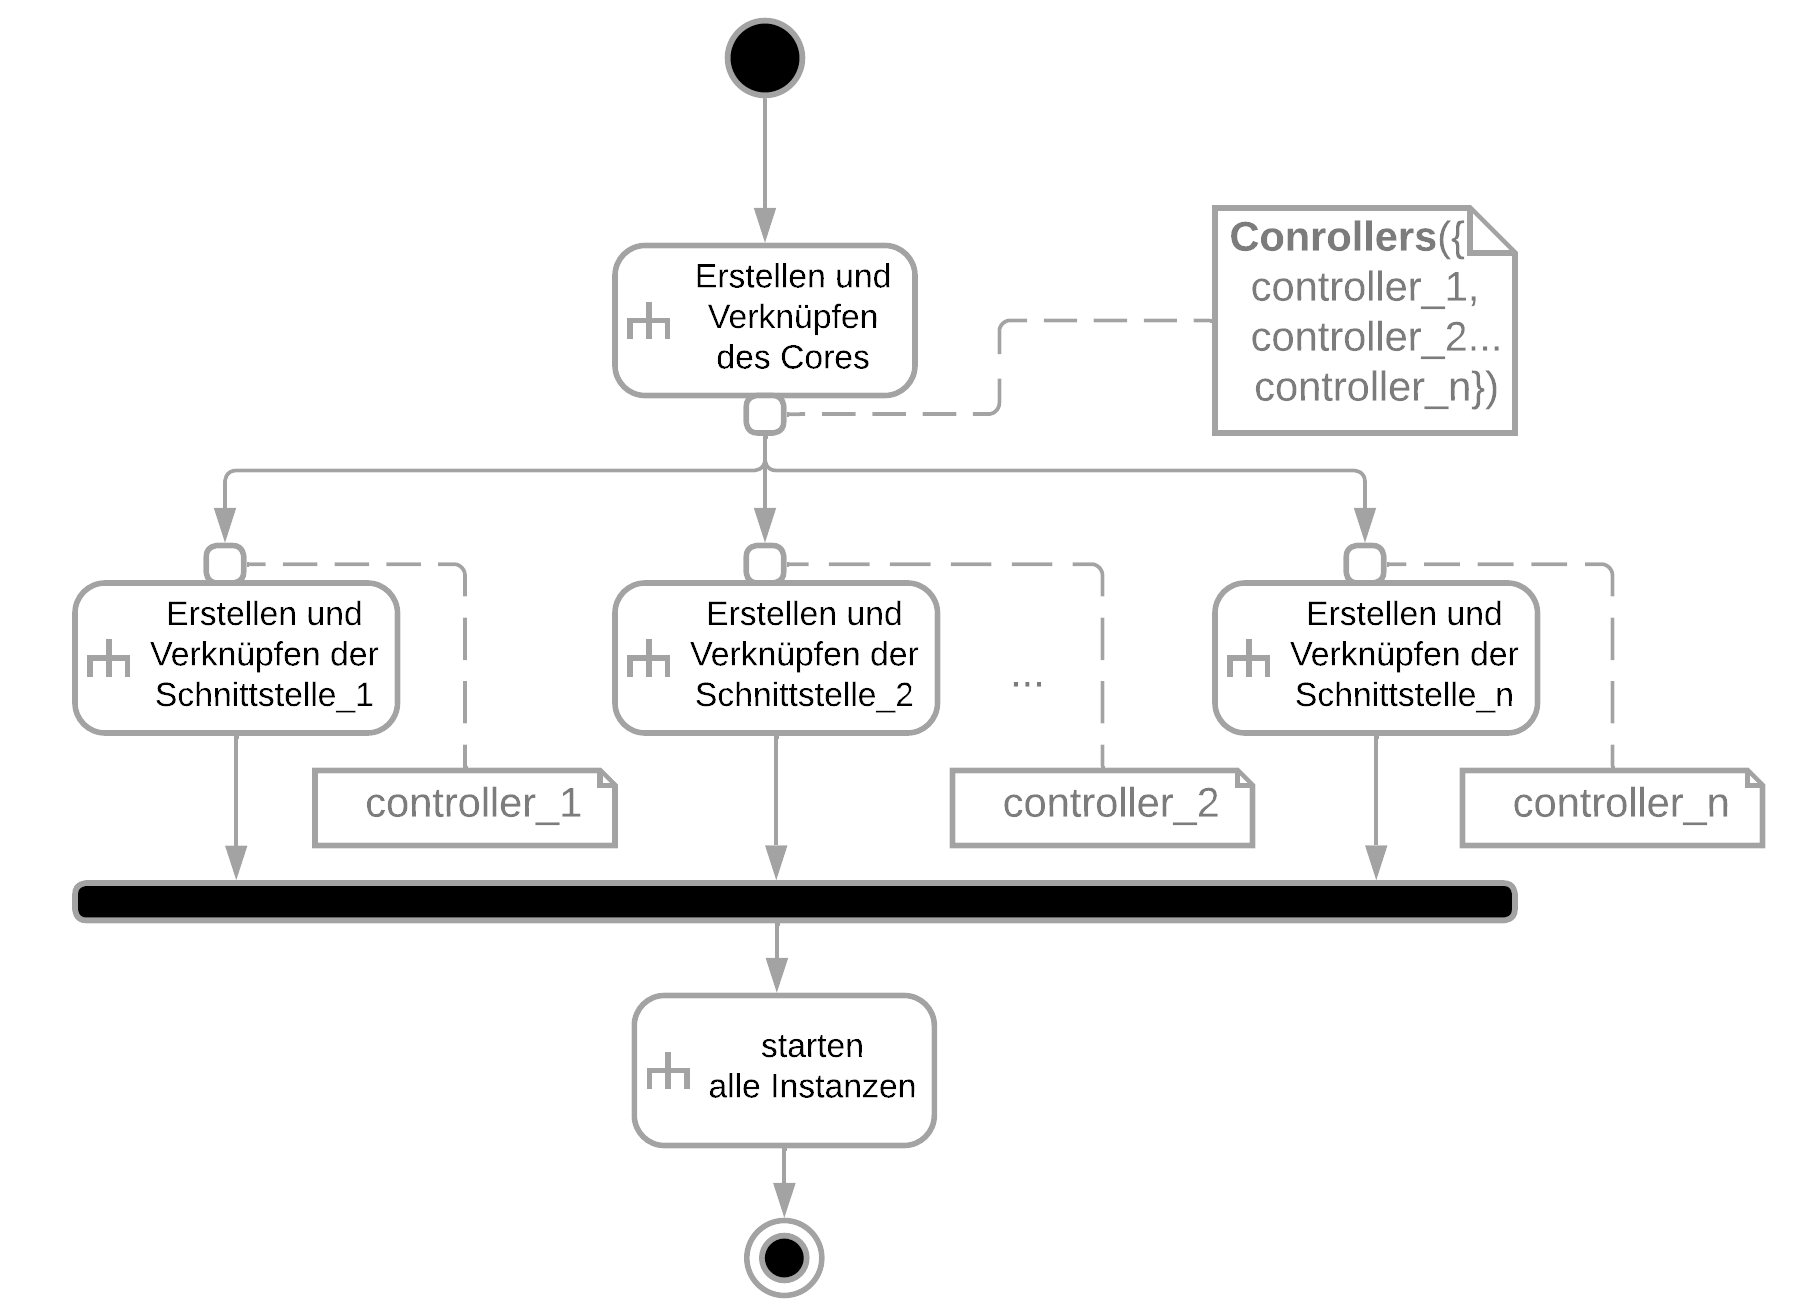
\includegraphics[width=12cm]{./images/Erstellen AD.png}
         \caption[Ablaufiagramm Erstellen der Struktur]{Ablaufiagramm Erstellen der Struktur \footnotemark}
         \label{fig:ADCreate}
    \end{figure}
    \footnotetext{Eigene Quelle}


    Mit diesem Ablauf können mehrere \textbf{Main}s erstellt werden, die verschiedene Anwendungen für verschiedene Zwecke erstellen.
    Z.B. ein Framework braucht keine reelen Anknüpfungen an die Infrastruktur (z.B. Datenbank) im Vergleich zu Standalone Anwendung.
    Oder es können verschiedene \textbf{Main}s für verschiedene Datenbanken.


    \subsubsection{Utility Controllers}
    zum Beispiel: Logger, Datum Error Fabrique

    \newpage
    \subsection{Datenfluss im Programm}
    Im System gibt es 3 wichtige Datenflusse, die durch Kombination miteinander die komplexen Abläufe im System umsetzen
    \begin{enumerate}
        \item (blau) Controller löst ein Ereignis im Dispatcher aus.
        \item (rot) Controller spricht sein Port an(z.B. Speichern der Daten in der Datenbank oder OCPP Antwort abzuschicken)
        \item (grün) Das Programm wird von einem externen System angesprochen (z.B. Ladesäule schickt eine OCPP Nachricht an den Server) 
    \end{enumerate}
    Wenn das geschehen ist, sieht der Datenfluss so aus:
    \import{./images/}{circle_2}
    \footnotetext{Eigene Quelle}

    \newpage
    Darstellung des Datenflusses \textbf{1} als \textbf{Sequencediagram}:

    \begin{figure}[h]
        \begin{sequencediagram}
            \newthread{A}{Controller 1}
            \newinst[1]{B}{Dispatcher}
            \newinst[1]{C}{UseCase}
            \newinst[1]{D}{Interactor I}
            \newinst[1]{E}{Controller J}
            
            \begin{messcall}{C}{subscribe ``Event''}{B}
            \end{messcall}

            \begin{messcall}{A}{Event}{B}{}
                    \begin{messcall}{B}{Event}{C}{}
                        \begin{sdblock}{Loop}{Until sequence of use case done}
                            \begin{call}{C}{Handle I}{D}{result}
                                \begin{call}{D}{Handle I}{E}{result}
                                \end{call}
                            \end{call}
                        \end{sdblock}
                    \end{messcall}
            \end{messcall}
          \end{sequencediagram}
          \caption{Sequencediagramm vom Datenfluss ``1'' Blau}
          \label{fig:seqDiagBlue}
    \end{figure}

    Wenn im \textbf{Controller} ein Ereignis erzeugt wird, wird \textbf{Dispatcher} darüber informiert. ein
    oder mehrere \textbf{UseCases} haben bereits dieses Event bei \textbf{Dispatcher} aboniert.
    \textbf{Dispatcher} informiert alle auf das Ereignis abonierte \textbf{UseCases}. 
    Jeder UseCases kann seinen eigenen Verhalten auf das Event definieren unabhängig voneinander.
    \textbf{UseCase} definiert einen Ablauf an \textbf{Interactoren},
    die wie vorgeschrieben ausgeführt werden. Jeder \textbf{Interactor} ruft eine Methode von einem \textbf{Controller} auf 
    und das Ergebnis wird an \textbf{UseCase} zurückgegeben, das vom UseCase entsprechend behandelt wird.

    \newpage
    Dabei es gibt 2 Möglichkeiten wie das Ereignis vom \textbf{Controller J} das \textbf{Interactor I} erreichen kann:
    \begin{enumerate}
        \item synchron - der Rückgabewert ist das Ergebnis der aufgerufenen Methode 
        \item asynchron - man wartet auf dazugehörige Antwort vom Port (z.B. auf OCPP Response warten, wenn man ein OCPP Request abschickt)
    \end{enumerate}

    Darstellung der 2. Möglichkeit:
    \begin{figure}[h]
        \begin{sequencediagram}
            \newthread{U}{UseCase}
            \newinst[1]{A}{Interactor I}
            \newinst[2]{C}{Dispatcher}
            \newinst[1]{B}{Controller J}
            \newthread{D}{...Externe}
            
            \begin{call}{U}{Message}{A}{Response}
            
            \begin{messcall}{A}{Message}{B}{}
                \begin{messcall}{A}{subscribe 'Response'}{C}{}
                    
                \end{messcall}
                \begin{messcall}{B}{Message}{D}{}
                \end{messcall}
            \end{messcall}
            \begin{messcall}{D}{Response}{B}{}
                \begin{messcall}{B}{Response}{C}{}
                    \begin{messcall}{C}{Response}{A}{}

                    \end{messcall}
                \end{messcall}

                \begin{messcall}{A}{unsubscribe 'Response'}{C}{}
                \end{messcall}
            \end{messcall}
            
                
            \end{call}
        \end{sequencediagram}
    \end{figure}

    Der Rückgabewert wird beim synchronen Funktionsaufruf zurückgegeben, wie in der Abbildung ~\ref{fig:seqDiagBlue} dargestellt.
    Der Rückgabewert beim asynchronen Funktionsaufruf, wird wie folgt definiert:
    Der Aufgerufene Interactor ruft eine Methode vom Controller auf, der die Nachricht an den externen Teilnehmer abschickt. 
    Gleich danach abonniert der Interactor die Antwort auf die abgeschickte Nachricht. Wenn die Antwort ankommt, landet sie beim Dispatcher,
    die alle Abonierten darüber informiert, unteranderem auch den Interactor. Der Interactor gibt diese Antwort als Rückgabewert der Funktionsaufruf

    \newpage
    Darstellung des Datenflusses ``2'' als ``sequencediagram'':
    \begin{figure}[h]
        \begin{sequencediagram}
            \newthread{A}{Controller}
            \newinst[1]{B}{Adapter}
            \newinst[1]{C}{Port}
            \newinst[3]{D}{Externe}
            \begin{call}{A}{Message}{B}{return result}
                \begin{call}{B}{Message}{C}{return result}
                    \begin{messcall}{C}{Message}{D}{}
                        
                    \end{messcall}
                \end{call}
            \end{call}
        \end{sequencediagram}
    \end{figure}\\
    Darstellung der Datentransformation:\\
    Controller - Adapter: Alle Informationen werden als Objekte übergeben, die im Domain definiert werden müssen.
    \begin{lstlisting}[language=json,firstnumber=1]
        OCPP20Message({
            destination: {
                chargerId : "some_unique_charger_id"
            },
            message : {
                name : "BootNotification",
                type : "Response",
                payload : BootNotification({
                    currentTime : Date(Thu Jul 28 2022 14:26:49 GMT+0200),
                    interval : 30,
                    status : "Rejected"    
                })
            }
        })
        \end{lstlisting}
        Adapter - Port: Alle Informationen, die gesendet werden (in dem Fall ``message''), werden in der verstandlichen Form (sie muss nicht mehr geändert werden)
        für den Port an Port weitergegeben.
        Über das Ziel müssen alle Informationen weitergegeben werden, so dass Port die entsprechende Verbindung zuordnen kann. 

        \begin{lstlisting}[language=json,firstnumber=1]
        {
            destination : {
                chargerId : "some_unique_charger_id"
            }
            message : "[3, 'message_id_of_request', {currentTime : 'Thu Jul 28 2022 14:26:49Z', interval : 30, status : 'Rejected'}]"
        }
    \end{lstlisting}


    Darstellung des Datenflusses ``3'' als ``sequencediagram'':
    \begin{figure}[h]
        \begin{sequencediagram}
            \newthread{A}{Externe}
            \newthread{B}{Port}
            \newinst{C}{Adapter}
            \newinst{D}{Controller}

            \begin{messcall}{A}{Message}{B}
                \begin{messcall}{B}{Message}{C}
                    \begin{messcall}{C}{Message}{D}
                        
                    \end{messcall}
                \end{messcall}
            \end{messcall}
        \end{sequencediagram}
    \end{figure}
    
    Beschreibung der Struktur des Programms:
    \textbf{hier kommt das Bild nur mit der Structur}
    \begin{itemize}
        \item 
    \end{itemize}



    \subsubsection{Auswahl der Datenbank}
    \subsubsection{Dependency Rule}
    \subsubsection{Unterschied zu Layered Architektur}
    \subsubsection{Implementierung der Testbarkeit}
    - Humble Objects
    \subsubsection{Dependency Injection}
    In der Abbildung \ref{fig:dateflowVScodedep} sieht man ein Beispiel von einer Anwendung, die die von der Konsole ankommenden Zahlen quadriert und das Ergebnis zurückgibt.
    
    \begin{figure}[H]
        \centering
        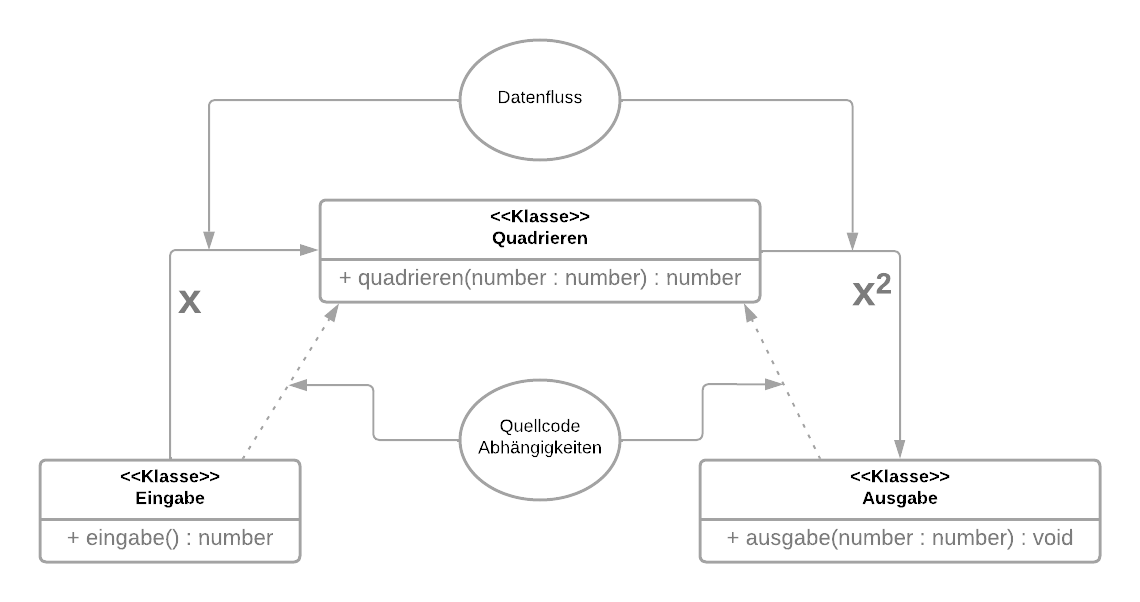
\includegraphics[width=1\textwidth]{./images/DepInj_1.png}
        \caption{Datenfluss und Quellcode Abhängigkeiten}
        \label{fig:dateflowVScodedep}
        \source{Eigene Quelle}
    \end{figure}

    Die Funktion \textbf{Quadrieren} ist in dem Fall befindet sich auf einem höheren Niveau als Eingabe und Ausgabe, 
    da das Quadrieren einer Zahl soll unabhängig von der Eingabe und Ausgabe sein.

    Würde man aber bei der Ausgabe die Eingabeparameter von \textbf{number} auf \textbf{string} ändern, 
    so müsste man auch die Ausgabe von Quadrieren von \textbf{number} auf \textbf{string} ändern.
    Dies könnte auch eine weitere Kette an Anderungen im Programm auslösen. 
    Zum Beispiel müssen auch die Unittests von \textbf{Quadrieren} geändert werden.
    Somit ist \textbf{Quadrieren} abhängig von der \textbf{Ausgabe}

    Das Problem lässt sich mittels Dependency Injection lösen.
    In OOP Sprachen kann man dafür ``Interface'' benutzen.

    Die Lösung wurde dann so aussehen. 
    \begin{figure}[H]
        \centering
        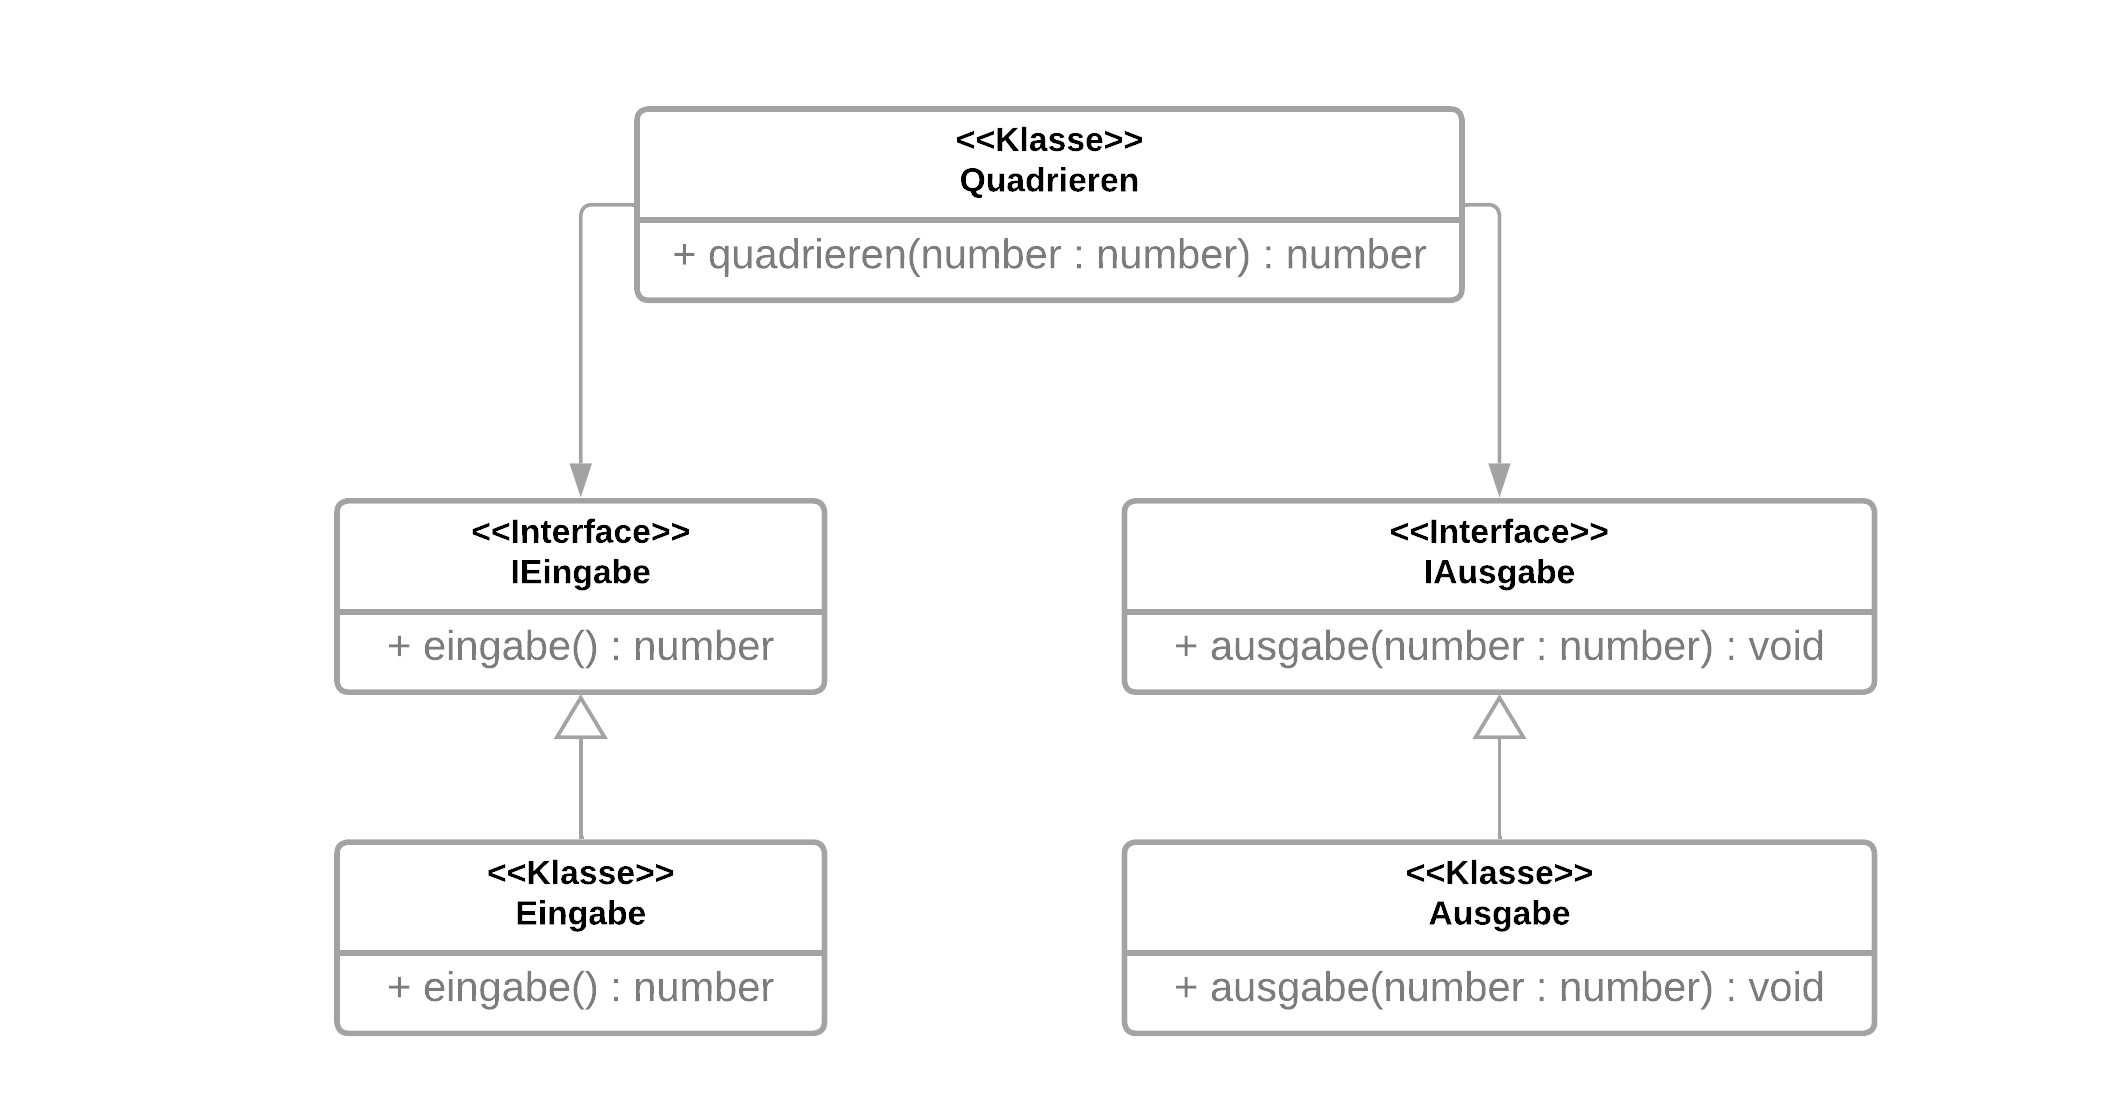
\includegraphics[width=1\textwidth]{./images/DepInj_2.png}
        \caption{Entkopplung der Abhängigkeiten}
        \label{fig:flow around cylinder}
        \source{Eigene Quelle}
    \end{figure}

    Dies lässt sich mit \textbf{Interface} (für OOP Sprachen) umsetzen, 
    in dem es frühestens bei der Initialisiereung der \textbf{Quadrieren} 
    Klasse das jeweilige Eingabe und Ausgabe Objekt übergeben wird.

    Somit lässt sich die Funktion \textbf{Quadrieren} mit gefälschten Eingabe- und Ausgabeklasse mit Unit tests getestet werden.

    Wenn man alle Klassen über Interface miteinander verbindet, 
    ist es möglich, dass die Umgebung von jeder einzelnen Klasse bei den Unittests gefälscht
    wird und somit das Schreiben von Unittests sehr einfach wird. 

    Interfaces können sich natürlich auch ändern und dann muss man auch alle davon betroffenen Objekte entsprechend ändern, 
    jedoch das passiert deutlich seltener als Änderung einer Klasse.

    Auch mit Dependency Injection lassen sich externe Schnittstellen wie Datenbank oder Netzwerkschnittstellen schnell austauschen, 
    denn man muss nur eine Klasse schreiben, die das Interface implementiert.
\newpage



% Example section added from an external tex-file, here located in ./Sections/
\import{./Sections/}{Aufgabestellung}

\import{./Sections/}{Loesung}


% Beschreibung der gewünschten Implementierung
\newpage
\import{./Sections/}{Bestinterface}

% Beschreibung der Implementierung der Software
\newpage
\import{./Sections/}{Implementierung}

\section{Übersichtsdiagramm}

% Example section added directly into the main-file
\section{Conclusion}
\textit{But the fact that some geniuses were laughed at does not imply that all who are laughed at are geniuses. They laughed at Columbus, they laughed at Fulton, they laughed at the Wright Brothers. But they also laughed at Bozo the Clown} -  \textcite{sagan_1993}.

% Printing bibliography
\newpage
\printbibliography[heading = bibintoc, title = Bibliography]    % 'bibintoc' inserts our bibliography into the table of contents

% Inserting appendix with separate settings
\addappendix
\import{./Appendices/}{example_appendix}

% End of document
\end{document}
